% title: 함수 그래프 두 개
% description: pgfplots로 y = f(x), y = g(x)를 한 좌표평면에 그린다. 축 이름·범례·격자·π 눈금. 함수식과 범위만 바꿔 쓴다
% packages: pgfplots
% libraries:
% 함수는 declare function에서 바꾼다. pgfplots의 삼각함수는 도(degree) 단위라 라디안은 sin(deg(x))로 쓴다.
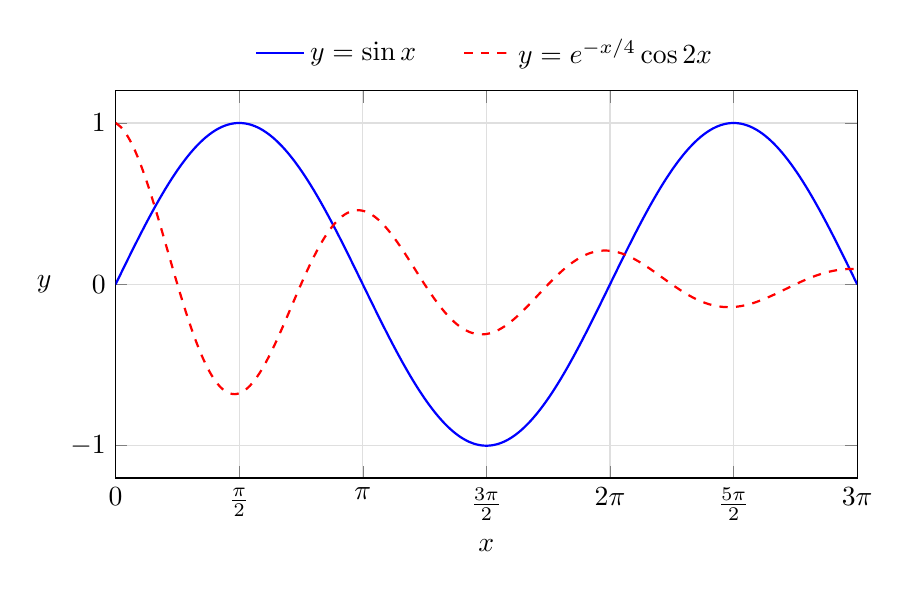
\begin{tikzpicture}[declare function={
    f(\x) = sin(deg(\x));
    g(\x) = exp(-\x/4)*cos(deg(2*\x));
  }]
  \begin{axis}[
      width=11cm, height=6.5cm,
      grid=major, grid style={gray!25},
      xmin=0, xmax=3*pi, ymin=-1.2, ymax=1.2,
      xtick={0, pi/2, pi, 3*pi/2, 2*pi, 5*pi/2, 3*pi},
      xticklabels={$0$, $\frac{\pi}{2}$, $\pi$, $\frac{3\pi}{2}$, $2\pi$, $\frac{5\pi}{2}$, $3\pi$},
      xlabel={$x$}, ylabel={$y$}, ylabel style={rotate=-90},
      domain=0:3*pi, samples=150, smooth,
      legend style={at={(0.5,1.03)}, anchor=south, draw=none,
                    /tikz/every even column/.append style={column sep=1.5em}},
      legend columns=2, legend cell align=left]
    \addplot[thick, blue] {f(x)};
    \addlegendentry{$y=\sin x$}
    \addplot[thick, red, dashed] {g(x)};
    \addlegendentry{$y=e^{-x/4}\cos 2x$}
  \end{axis}
\end{tikzpicture}
